% fcs_mpc_ttype_psm.tex
% Finite-set predictive current control of the three-level T-type inverter of a PM wind generator (model
% mpc_ttype_psm of modelization-and-control): what was wrong in the model, the fixes and their verification.
% pwr-control template (AAA_template_latex_settings); numbers and figures: fcs_mpc_ttype_psm_analysis.py
% (python3, numpy, matplotlib). Compile: pdflatex fcs_mpc_ttype_psm.tex (three times, for references).
% Rev. 00 - November 2026 - first issue
\documentclass[10pt,a4paper]{scrartcl}
% ===================== PACKAGES =====================
\usepackage[british]{babel}
\usepackage[tmargin=1in, bmargin=1in, lmargin=0.75in, rmargin=0.75in]{geometry}
\usepackage[dvipsnames,table]{xcolor}  % prima di tikz, listings, ecc.

\usepackage{tikz}
\usepackage{graphicx}
\usepackage{pgfplots}
\pgfplotsset{width=12cm, compat=1.9}
\usepackage{setspace}
\usepackage{chemmacros}
\usepackage{chemfig}
\usepackage{esint}
\usepackage{tabularray}
\usepackage{makeidx}
\usepackage{epstopdf}
\usepackage{amssymb}
\usepackage{mathrsfs}
\usepackage{bm}
\usepackage{amsmath}
\usepackage{enumitem}
\usepackage[english]{varioref}
\usepackage{lipsum}
\usepackage{fancyhdr}
\usepackage{float}
\usepackage{empheq}
\usepackage[framemethod=tikz]{mdframed}
\numberwithin{equation}{section}
\usepackage{eso-pic}
\usepackage{calc}
\usepackage{nccmath}
\usepackage{caption}
\usepackage{subcaption}
\usepackage{gensymb}
\usepackage{amsfonts, amsthm, epsfig, epstopdf, titling, url, array}
\usepackage{tabularx}
\usepackage{makecell}
\usepackage{booktabs}
\usepackage{array}
\usepackage{siunitx}
\sisetup{input-digits=0123456789\pi}
\usepackage[symbol]{footmisc}
\usepackage{multicol}
\usepackage{boondox-cal}
\usepackage{blindtext}
\usepackage{changepage}
\usepackage{nomencl}
\usepackage{hyperref}
\usepackage{xurl}
\usepackage{ragged2e}
\usepackage[version=4]{mhchem}  % ← conflitto di opzioni
\usepackage{longtable}
\usepackage{chemformula}
\usetikzlibrary{arrows.meta,positioning,calc}

% ===================== SI UNITS =====================
\DeclareSIUnit\atm{atm}
\DeclareSIUnit{\var}{var}
\DeclareSIUnit{\pu}{p.u.}


% ===================== MATH OPERATORS =====================
\DeclareMathOperator{\rank}{rank}
\DeclareMathOperator{\atantwo}{atan2}
\DeclareMathOperator{\spn}{span}

% ===================== COMMANDS =====================
\newcommand{\abs}[1]{\left|#1\right|}
\newcommand{\sign}{\text{sign}}
\newcommand{\centered}[1]{\begin{tabular}{@{}l@{}} #1 \end{tabular}}

% ===================== COLORS =====================
\definecolor{mycolor1}{rgb}{0.97, 0.97, 0.97}
\definecolor{mycolor2}{rgb}{0.97, 0.97, 0.97}
\definecolor{tableShade}{gray}{0.9}

% ===================== THEOREM ENVIRONMENTS =====================
\theoremstyle{it}
\newtheorem{defn}{Definition}[section]
\newtheorem{assumption}{Assumption}[section]
\newtheorem{thm}{Theorem}[section]
\newtheorem{lemma}{Lemma}[section]
\newtheorem{corollary}{Corollary}[section]
\theoremstyle{definition}
\newtheorem{example}{Example}[section]

% ===================== CUSTOM ENVIRONMENTS =====================
\newenvironment{myitemize_1}{
	\begin{itemize}[topsep=0pt]
		\setlength{\topsep}{2pt}
		\setlength{\itemsep}{2pt}
		\setlength{\parskip}{2pt}
		\setlength{\parsep}{2pt}
	}{\end{itemize}}

\newmdenv[
innerlinewidth=0.5pt,
roundcorner=4pt,
backgroundcolor=mycolor2,
linecolor=mycolor1,
innerleftmargin=6pt,
innerrightmargin=6pt,
innertopmargin=6pt,
innerbottommargin=6pt
]{mybox}

% ===================== TABLE COLUMN TYPES =====================
\newcolumntype{Y}{>{\hsize=2\hsize}X}
\newcolumntype{Z}{>{\centering\arraybackslash\hsize=0.857\hsize}X}

% ===================== SECTION DEPTH =====================
\setcounter{secnumdepth}{3}
\setcounter{tocdepth}{3}

% ===================== PAGE STYLE =====================
\setlength{\headheight}{20pt}
\setlength{\headsep}{20pt}

\pagestyle{fancy}
\fancypagestyle{firstpage}{\rhead{}}
\fancyhead[L]{\slshape\nouppercase{\leftmark}}
\chead{}
\rhead{\includegraphics[height=0.75cm]{../../AAA_template_latex_settings/pwr-control_logo_doc.png}}
\lfoot{\href{http://www.pwr-control.com}{pwr-control.com}}
\cfoot{-\ \thepage\ -}
\rfoot{\textit{}}
\renewcommand{\headrulewidth}{0.4pt}
\renewcommand{\footrulewidth}{0.4pt}


\geometry{
	a4paper,
	top    = 2.5cm,
	bottom = 3.0cm,
	left   = 2.5cm,
	right  = 2.5cm
}

\hypersetup{
	colorlinks = true,
	urlcolor   = blue,
	linkcolor  = black,
	citecolor  = black
}

\pagenumbering{gobble}
% the document sits three levels below the repository root: logo path of settings.tex corrected here
\rhead{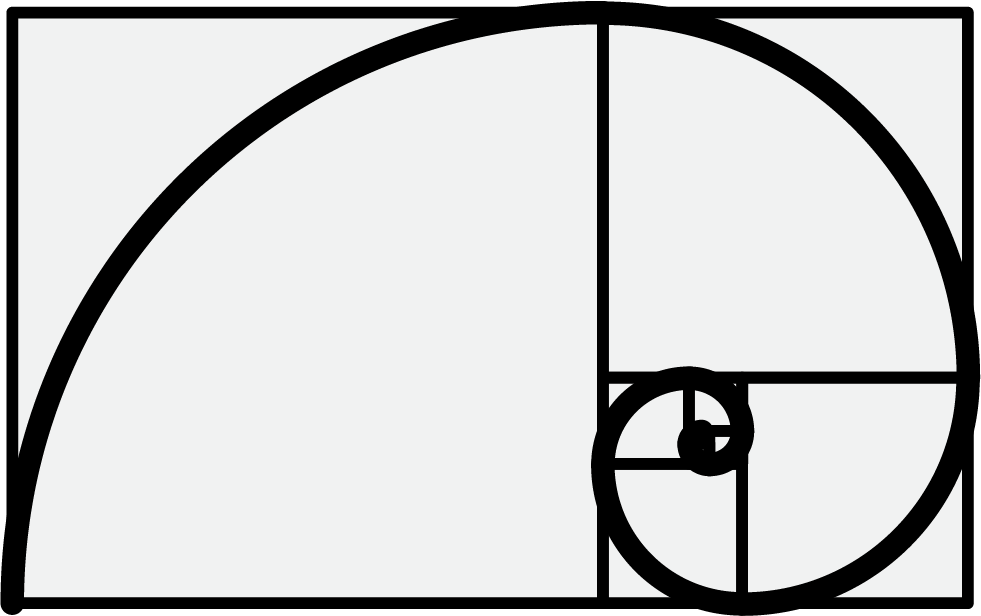
\includegraphics[height=0.75cm]{../../../AAA_template_latex_settings/pwr-control_logo_doc.png}}
\rfoot{\small Rev.~00}
\geometry{left=2.0cm, right=2.0cm}
\usetikzlibrary{arrows.meta,positioning}

\sisetup{per-mode=symbol,range-phrase={\text{--}},range-units=single,retain-explicit-plus}
\setlist{nosep}
\setlength{\parindent}{0pt}
\setlength{\parskip}{3pt}
\allowdisplaybreaks

% --- shorthand ---
\newcommand{\ts}{t_s}
\newcommand{\tspu}{\tau_s}
\newcommand{\jj}{\mathrm{j}}
\newcommand{\ee}{\mathrm{e}}
\newcommand{\pu}{\,\mathrm{pu}}
\newcommand{\code}[1]{\texttt{#1}}
\newcommand{\ub}{u_{bez}}
\newcommand{\ib}{i_{bez}}
\newcommand{\wb}{\omega_{bez}}
\newcommand{\udcn}{u_{dc,nom}}

% =============================================================
%  DOCUMENT DATA (title page: AAA_template_latex_settings/titlepage.tex)
% =============================================================
\newcommand{\DocCategory}{Technical Note}
\newcommand{\DocField}{Power Electronics and Control Systems}
\newcommand{\DocTitle}{%
	{\fontsize{20}{24}\selectfont\bfseries Finite-Set Predictive Current Control} \\[12pt]
	{\fontsize{16}{26}\selectfont\bfseries of a T-Type Wind-Generator Inverter: \\[8pt] analysis and fixes of the model \texttt{mpc\_ttype\_psm}}
}
\newcommand{\DocSubtitle}{Voltage base and delay compensation of the prediction, neutral point and switching terms, \\[6pt] voltage, inductance and speed of the EKF, gate overlap of the T-type legs}
\newcommand{\DocAuthor}{Davide Bagnara}
\newcommand{\DocRevision}{00}
\newcommand{\DocDate}{November 2026}
\newcommand{\DocAbstract}{%
The model \texttt{mpc\_ttype\_psm} simulates one of the six systems of a \SI{1.6}{MW}, \SI{17.8}{rpm} permanent magnet wind generator on a three-level T-type inverter with a split DC link across a battery. A finite-set model predictive control (FCS-MPC) tests the 27 states of the bridge every \SI{125}{\micro s} and an extended Kalman filter (EKF) gives angle, flux and speed without sensor. A switched simulation of the whole chain showed that the control worked far from its design: torque \SI{11.5}{\percent} below the torque curve, angle error \ang{-21.6}, a large current ripple, the neutral point of the DC link not controlled and a possible one-step short circuit of a DC-link capacitor at each change from the neutral point to a rail. This note explains the causes (voltage base of the prediction, missing delay compensation, neutral-point term, ties between redundant states, voltage, inductance and state prediction of the EKF, speed bias, gate interlock of the T-type legs), gives the eleven fixes now in the model and their verification: with the fixes the torque is on the curve within \SI{0.4}{\percent}, the angle error is \ang{-1.2}, the current error is one third, the neutral point stays within \SI{\pm 9}{V} and the switches no longer overlap. A companion Python script reproduces every number and figure.
}
\newcommand{\RevisionHistory}{%
	00 & November 2026 & First issue. & \DocAuthor \\
}
\newcommand{\MetaLabelA}{Project Repository}
\newcommand{\MetaValueAUrl}{https://github.com/pwr-control/modelization-and-control.git}
\newcommand{\MetaValueALabel}{modelization-and-control.git (foundations\_of\_power\_electronics/mpc\_ttype\_psm)}
\newcommand{\MetaLabelB}{Framework}
\newcommand{\MetaValueB}{MATLAB/Simulink/Simscape; Python 3 (\texttt{fcs\_mpc\_ttype\_psm\_analysis.py})}

\begin{document}
% =============================================================
%  pwr-control LaTeX template - FRONTESPIZIO
%
%  Da richiamare come prima istruzione dopo \begin{document}:
%      \input{../../AAA_template_latex_settings/titlepage}
%
%  Il documento deve definire prima di \begin{document}:
%      \DocCategory   categoria del documento
%      \DocField      area tecnica
%      \DocTitle      titolo (una o due righe)
%      \DocSubtitle   sottotitolo
%      \DocAuthor     autore/i, separati da virgola
%      \DocRevision   numero di revisione corrente (es. 00)
%      \DocDate       data della revisione corrente
%      \DocAbstract   abstract
%      \RevisionHistory  righe della tabella di revisione, nel formato
%                        Rev. & Date & Description & Authors \\
%      \MetaLabelA \MetaValueAUrl \MetaValueALabel
%      \MetaLabelB \MetaValueB
% =============================================================

\providecommand{\DocCategory}{Technical Research Report}
\providecommand{\DocField}{Power Electronics and Control Systems}
\providecommand{\DocSubtitle}{}
\providecommand{\DocRevision}{00}
\providecommand{\DocAbstract}{}
\providecommand{\RevisionHistory}{%
	\DocRevision & \DocDate & First issue. & \DocAuthor \\
}

\titlepage

% ---- Intestazione centrata ----
\begin{center}
	{\Large\scshape \DocCategory}\\[8pt]
	{\large\scshape \DocField}
\end{center}

\vspace{30pt plus 4pt minus 14pt}
\noindent\rule{\linewidth}{0.8pt}

% ---- Titolo ----
\begin{center}
	\DocTitle
\end{center}

\vspace{4pt}
\noindent\rule{\linewidth}{2.2pt}

% ---- Sottotitolo ----
\begin{center}
	\begin{onehalfspace}
		{\large\itshape \DocSubtitle}
	\end{onehalfspace}
\end{center}

% ---- Authors / Revision / Date ----
\vspace{30pt plus 4pt minus 14pt}

\noindent
\begin{minipage}[t]{0.46\linewidth}
	\raggedright
	\textbf{Authors:}\\[2pt]
	\DocAuthor
\end{minipage}%
\hfill
\begin{minipage}[t]{0.22\linewidth}
	\centering
	\textbf{Revision:}\\[2pt]
	\DocRevision
\end{minipage}%
\hfill
\begin{minipage}[t]{0.30\linewidth}
	\raggedleft
	\textbf{Date:}\\[2pt]
	\DocDate
\end{minipage}

\vspace{10pt}
\noindent\rule{\linewidth}{0.8pt}

% ---- Abstract ----
\vspace{24pt plus 4pt minus 12pt}

\begin{center}
	\begin{minipage}{0.88\linewidth}
		\footnotesize
		\begin{onehalfspace}
			\textbf{Abstract:} \DocAbstract
		\end{onehalfspace}
	\end{minipage}
\end{center}

\vfill

% ---- Revision history ----
\begin{center}
	\begin{minipage}{0.96\linewidth}
		\centering
		{\footnotesize\scshape Revision history}\\[6pt]
		{\footnotesize
			\begin{tabular}{@{}cl>{\raggedright\arraybackslash}p{0.36\linewidth}>{\raggedright\arraybackslash}p{0.28\linewidth}@{}}
				\toprule
				\textbf{Rev.} & \textbf{Date} & \textbf{Description} & \textbf{Authors} \\
				\midrule
				\RevisionHistory
				\bottomrule
			\end{tabular}}
	\end{minipage}
\end{center}

\vspace{18pt plus 4pt minus 10pt}

% ---- Metadati in fondo ----
\noindent
\begin{tabular}{@{} r @{\quad} l @{}}
	\textsc{\MetaLabelA:} & {\href{\MetaValueAUrl}{\MetaValueALabel}} \\[3pt]
	\textsc{\MetaLabelB:} & {\MetaValueB}       \\[3pt]
\end{tabular}

% =============================================================
%  Fine frontespizio
% =============================================================
\newpage
\pagenumbering{arabic}
\setcounter{page}{1}

\tableofcontents
\newpage
\begin{onehalfspace}

% =====================================================================================================
\section{Scope}
\label{sec:scope}

The model \code{mpc\_ttype\_psm} (\path{foundations_of_power_electronics/mpc_ttype_psm} of modelization-and-control) simulates one of the six three-phase systems of a \SI{1.6}{MW}, \SI{17.8}{rpm}, 104-pole permanent magnet synchronous generator (about \SI{267}{kW} per system). The system feeds a three-level T-type inverter with ideal switches through a \SI{230}{\micro H} inductor; the split DC link ($2\times\SI{14.4}{mF}$, neutral point O at the centre tap) sits across a \SI{1200}{V} lithium-ion battery. The shaft turns at a fixed speed, the torque reference comes from the torque curve of the turbine, the current reference is on the q axis only ($i_d = 0$) and a finite-set model predictive control (FCS-MPC) \cite{kouro2009,rodriguez2012} chooses one of the 27 states of the bridge every control step and writes the twelve gate commands directly. A six-state EKF \cite{bolognani1999} gives the rotor angle, the magnet flux and the speed.

During the migration of the model to the parameter structure of the repository (November 2026) a switched simulation of the whole chain showed that the control worked far from its design. This note collects the analysis and the fixes, which are now in the model (pull request \#25 of modelization-and-control): Sect.~\ref{sec:system} gives the per-unit chain and the timing, Sect.~\ref{sec:mpc} the predictive control, Sect.~\ref{sec:observers} the observers, Sect.~\ref{sec:gates} the gate timing of the T-type legs, Sect.~\ref{sec:verification} the verification and Sect.~\ref{sec:open} the remaining points. Every number comes from the companion script \code{fcs\_mpc\_ttype\_psm\_analysis.py} (same data and formulas as \code{init\_model.m} of the model). The fixed model was then run in MATLAB/Simulink (1 November 2026) and runs well. An FPGA implementation of an FCS-MPC for a T-type inverter with an RL load is described in the note \path{research/power_electronics/mpc_three_phase_ttype_inverter_fpga} of this repository.

% =====================================================================================================
\section{System, per unit and timing}
\label{sec:system}

\subsection{Data and per-unit bases}

The control works in the per unit of the machine (one system): voltages in $\ub$ (peak phase voltage), currents in $\ib$ (peak phase current), time in $1/\wb$, flux in $\ub/\wb$, inductances in $L_{bez} = \ub/(\ib\wb)$. The DC voltages come from the DC-link block in per unit of $\udcn = \SI{1070}{V}$ (the base of the \SI{690}{V} hardware data set). Table~\ref{tab:data} lists the data.

\begin{table}[htb]
\centering
\caption{Data of one system and of the control (values of \code{init\_model.m}).}
\label{tab:data}
\small
\begin{tabularx}{\textwidth}{@{}l>{\raggedright\arraybackslash}Xl@{}}
\toprule
Quantity & Value & Per unit \\
\midrule
bases & $\ub = \SI{365.8}{V}$, $\ib = \SI{486.0}{A}$, $\wb = \SI{96.93}{rad/s}$ (\SI{15.43}{Hz}), $L_{bez} = \SI{7.77}{mH}$ & \\
machine & $R_s = \SI{30.1}{m\ohm}$, $L_d = \SI{6.24}{mH}$, $L_q = \SI{7.56}{mH}$, $\psi_m = \SI{3.774}{Vs}$ & 0.040, 0.804, 0.974, 1.000 \\
output inductor & $L_{Fi} = \SI{230}{\micro H}$, $R_{LFi} = \SI{1.8}{m\ohm}$ & 0.030 \\
seen by the bridge & $L_d + L_{Fi}$, $L_q + L_{Fi}$, $R_s + R_{LFi}$ & 0.833, 1.003, 0.042 \\
DC link & $2\times\SI{14.4}{mF}$; battery \SI{1249}{V} open circuit (soc 0.85), \SI{1275}{V} while charging & 1.168 of $\udcn$ \\
control & $\ts = \SI{125}{\micro s}$ (\SI{4}{kHz} timer, double update), clock gain 1.001 & $\tspu = \ts\wb = 0.01212$ \\
rated point & \SI{17.8}{rpm}, torque curve \SI{125}{kNm}, \SI{233}{kW}, bridge voltage \SI{476}{V} peak & $i_q^* = -0.874$, $u = 1.30$ \\
\bottomrule
\end{tabularx}
\end{table}

Seen from the bridge, the machine and the inductor obey, in the stationary frame with complex space vectors ($\vec x = x_\alpha + \jj x_\beta$, amplitude-invariant Clarke transformation) and in per unit,
\begin{equation}
L\,\frac{\mathrm{d}\vec i}{\mathrm{d}\tau} = \vec u - R\,\vec i - \vec e, \qquad \vec e = \jj\,\omega\,\vec\psi,
\label{eq:plant}
\end{equation}
with $\tau = \wb t$, $\vec\psi$ the flux that rotates with the rotor (Sect.~\ref{sec:activeflux}) and $\omega$ the electrical speed. The prediction is the forward-Euler step of \eqref{eq:plant} over one control step:
\begin{equation}
\vec i_{k+1} = \vec i_k + g\,\big(\vec u_k - R\,\vec i_k - \vec e_k\big), \qquad g = \frac{\tspu}{L}.
\label{eq:pred}
\end{equation}

\subsection{Timing of the control}

Fig.~\ref{fig:timing} shows the timing. The currents and the DC voltages are sampled at $t_{k-1}$ and used at step $k$ (one step of acquisition delay); the vector $\vec u_k$ chosen at step $k$ acts over $[t_k, t_{k+1})$, so it decides the current at $t_{k+1}$. The current measured at step $k$ was made by $\vec u_{k-2}$, and the vector $\vec u_{k-1}$ is already acting when $\vec u_k$ is chosen. The control clock runs \SI{0.1}{\percent} fast (gain 1.001 of the local timing block), while the constants use $\ts = \SI{125}{\micro s}$.

\begin{figure}[htb]
\centering
\begin{tikzpicture}[x=2.9cm,y=1cm,>=Stealth,font=\small]
\draw[->] (-0.25,0) -- (4.35,0) node[right]{$t$};
\foreach \x/\l in {0/t_{k-2},1/t_{k-1},2/t_k,3/t_{k+1},4/t_{k+2}} {\draw (\x,0.08) -- (\x,-0.08) node[below]{$\l$};}
\fill[blue!12] (0,0.25) rectangle (1,0.75); \node at (0.5,0.5) {$\vec u_{k-2}$};
\fill[blue!12] (1,0.25) rectangle (2,0.75); \node at (1.5,0.5) {$\vec u_{k-1}$};
\fill[orange!30] (2,0.25) rectangle (3,0.75); \node at (2.5,0.5) {$\vec u_{k}$};
\draw[white,line width=1pt] (1,0.25) -- (1,0.75) (2,0.25) -- (2,0.75);
\draw[->,thick] (1,1.15) -- (1,0.8);
\node[above,align=center] at (1,1.15) {sample $\vec i$, $v_{dc1}$, $v_{dc2}$};
\node[draw,rounded corners,align=left,fill=white] (stepk) at (2.75,2.35) {step $k$: \textbf{1.} $\hat{\vec i}(t_k)$ from $\vec i(t_{k-1})$ and $\vec u_{k-1}$;\\ \textbf{2.} choose $\vec u_k$ for $\vec i(t_{k+1})$; \textbf{3.} give $\vec u_{k-2}$ to the EKF};
\draw[->] (1,1.65) to[out=70,in=180] (stepk.west);
\draw[->,dashed] (2,0 |- stepk.south) -- (2.0,0.8);
\draw[<->] (2,-0.55) -- node[below]{acts} (3,-0.55);
\end{tikzpicture}
\caption{Timing of one control step: samples taken at $t_{k-1}$ are used at step $k$; the vector chosen at step $k$ acts over the next step.}
\label{fig:timing}
\end{figure}

% =====================================================================================================
\section{The predictive control}
\label{sec:mpc}

\subsection{Voltage of a state}
\label{sec:voltage}

A state is $s = (s_a, s_b, s_c)$ with $s_x \in \{1, 0, -1\}$ (leg at P, O or N). With $v_{dc1}$ and $v_{dc2}$ the voltages of the upper and lower capacitors (per unit of $\udcn$), the leg voltage to the neutral point is $v_x = v_{dc1}$, $0$ or $-v_{dc2}$, and the voltage vector in the per unit of the machine is
\begin{equation}
u_\alpha = k_u\,\tfrac23\big(v_a - \tfrac12 v_b - \tfrac12 v_c\big), \qquad
u_\beta = k_u\,\tfrac{1}{\sqrt3}\big(v_b - v_c\big), \qquad k_u = \frac{\udcn}{\ub} = 2.925 .
\label{eq:ustate}
\end{equation}
\textbf{Before the fix} the code used $(v_{dc1} + v_{dc2})/3$ times the state pattern, i.e. a voltage in per unit of $\udcn$, in the model \eqref{eq:pred} written in per unit of $\ub$: the true voltage of every state was $k_u = 2.925$ times the predicted one (fix 1: the factor $k_u$, parameter \code{u\_scale}). Taking $v_{dc1}$ and $v_{dc2}$ apart also gives the right voltage when the neutral point is not centred.

\subsection{Delay compensation and the current loop}
\label{sec:deadbeat}

Without the vector limit, the choice of the state with the smallest current error is a deadbeat controller. On one axis, with $R$ and $\vec e$ compensated, let $b = \tspu/L_{true}$ be the true gain from the voltage to the current change and $\hat b$ the gain used by the prediction (including the voltage error of Sect.~\ref{sec:voltage}); call $g = b/\hat b$ the loop gain and $\varepsilon = i^* - i$ the error.

\textbf{Before the fix} the prediction started from the measured current $i_{k-1}$, so $u_k = (i^* - i_{k-1})/\hat b$ and
\begin{equation}
\varepsilon_{k+1} = \varepsilon_k - g\,\varepsilon_{k-1}, \qquad z^2 - z + g = 0, \qquad |z| = \sqrt g .
\label{eq:nocomp}
\end{equation}
Even with $g = 1$ the poles are on the unit circle (undamped oscillation at $f_s/6 = \SI{1.3}{kHz}$); with the voltage base of Sect.~\ref{sec:voltage} $g = 2.59$ on the q axis and 3.12 on the d axis, $|z| = 1.61$ and 1.77. The finite set of vectors keeps the current bounded, but the control picks vectors that are too large: a large ripple, few states with a leg at O and thousands of direct P$\leftrightarrow$N changes per second.

\textbf{With the delay compensation} (fix 2) \cite{cortes2012} the control first computes the current of now with the vector that is acting, $\hat\imath_k = i_{k-1} + \hat b\,u_{k-1}$ (with $R$ and $\vec e$ in the vector form \eqref{eq:pred}), and then chooses $u_k$ for $i_{k+1}$. Since $i_k = i_{k-1} + b\,u_{k-1}$,
\begin{equation}
\varepsilon_{k+1} = (1 - g)\,\varepsilon_{k-1}, \qquad z^2 = 1 - g ,
\label{eq:comp}
\end{equation}
deadbeat for $g = 1$ and stable for $0 < g < 2$. The prediction uses $L = L_q + L_{Fi}$ (Sect.~\ref{sec:activeflux}) on both axes, so $g = 1.000$ on the q axis and $g = (L_q + L_{Fi})/(L_d + L_{Fi}) = 1.204$ on the d axis: there the error is multiplied by $-0.204$ every two steps. The neutral-point voltage is advanced in the same way (Sect.~\ref{sec:np}).

\subsection{Neutral point}
\label{sec:np}

With equal capacitors $C$, the current $i_O$ that leaves the neutral point towards the legs at O (the sum of the phase currents of those legs) moves the difference of the two capacitor voltages, while the battery current loads both capacitors equally:
\begin{equation}
C\,\frac{\mathrm{d}(v_{dc1} - v_{dc2})}{\mathrm{d}t} = i_O
\quad\Rightarrow\quad
\Delta(v_{dc1} - v_{dc2}) = k_{np}\, i_O\, \tspu, \qquad k_{np} = \frac{\ib}{C\,\udcn\,\wb} = 0.325,
\label{eq:np}
\end{equation}
in per unit of $\udcn$ and $\ib$: one per unit of $i_O$ for one step moves $v_{dc1} - v_{dc2}$ by 0.0039 (\SI{4.2}{V}). \textbf{Before the fix} the term was written with a fictitious capacitance $10^{-3}$ in the per-unit time ($1/10^{-3}$ in place of $k_{np}$, 3070 times too strong) and its weight was $k_{dc} = 0$. Without the term, the redundant small vectors (P-type and N-type, same voltage, opposite $i_O$) give the same current error, the choice between them ignores $i_O$ and the neutral point is not controlled: over the \SI{1.5}{s} of the check $v_{dc1} - v_{dc2}$ wanders up to \SI{137}{V} in the model before the fix and swings by up to \SI{158}{V} in the fixed model without the term (case D1 of Sect.~\ref{sec:verification}, Fig.~\ref{fig:np}). Fix 3: $k_{np}$ as in \eqref{eq:np} and $k_{dc} = 1$; the term then has the same size as the current error and keeps $v_{dc1} - v_{dc2}$ within \SI{\pm 9}{V} \cite{vargas2007}.

\subsection{Switching term}
\label{sec:switching}

Several states give almost the same current: the three zero vectors (PPP, OOO, NNN) and the pairs of redundant small vectors. Without a switching term the order of the table decides, and a leg often jumps directly between P and N (a full DC-voltage step on the phase). The fixed cost function counts the level changes of the three legs from the applied state $s^-$,
\begin{equation}
N_{sw} = \sum_{x = a,b,c} |s_x - s_x^-| \qquad (\text{O}\leftrightarrow\text{P},\ \text{O}\leftrightarrow\text{N}: 1; \ \text{P}\leftrightarrow\text{N}: 2),
\label{eq:nsw}
\end{equation}
with the weight $k_{sw} = 10^{-5}$ (fix 4). The weight equals the cost of a current error of $\sqrt{10^{-5}} = 0.003\pu$, so it only breaks the ties. Fig.~\ref{fig:switching} and Table~\ref{tab:switching} show its effect: at \SI{17.8}{rpm} the switching per device halves and the P$\leftrightarrow$N changes drop from 812 to 108 per second; at \SI{12}{rpm} (partial load, many zero and small vectors) they drop from 4655 to 24 per second, while the current error at rated speed grows only from 0.0081 to $0.0083\pu$.

\begin{table}[htb]
\centering
\caption{Effect of the switching term (fixed model, sensorless). Switching per device: level changes of a leg per second divided by two, i.e. the switching frequency of the two switches that commutate (two of the four switches of a T-type leg commutate at a time; a carrier PWM with the same changes has this carrier frequency).}
\label{tab:switching}
\small
\begin{tabular}{lcccc}
\toprule
Case & current error rms & P$\leftrightarrow$N changes/s & switching per device & leg at O \\
\midrule
\SI{17.8}{rpm}, $k_{sw} = 0$ & 0.0081 pu & 812 & \SI{2712}{Hz} & \SI{45}{\percent} \\
\SI{17.8}{rpm}, $k_{sw} = 10^{-5}$ & 0.0083 pu & 108 & \SI{1532}{Hz} & \SI{47}{\percent} \\
\SI{12}{rpm}, $k_{sw} = 0$ & 0.0042 pu & 4655 & \SI{2878}{Hz} & \SI{33}{\percent} \\
\SI{12}{rpm}, $k_{sw} = 10^{-5}$ & 0.0042 pu & 24 & \SI{1429}{Hz} & \SI{51}{\percent} \\
\bottomrule
\end{tabular}
\end{table}

\begin{figure}[htb]
\centering
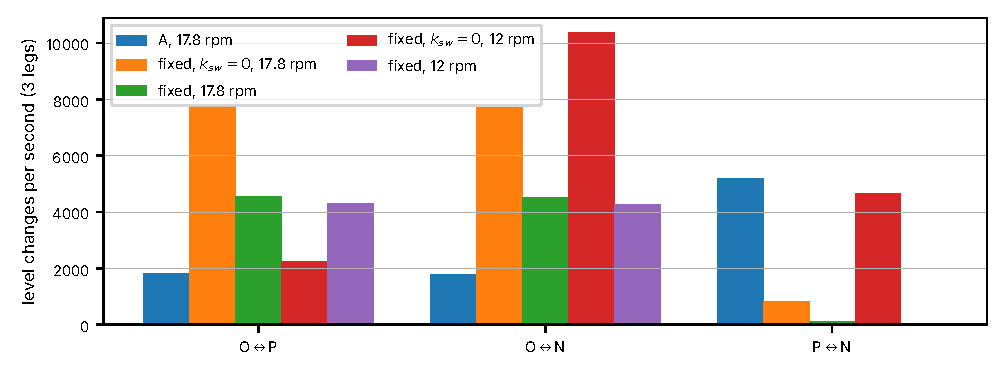
\includegraphics[width=\textwidth]{figures/fig_switching.pdf}
\caption{Level changes per second of the three legs, model before the fix (A) and fixed model with and without the switching term.}
\label{fig:switching}
\end{figure}

\subsection{Cost function and algorithm}

The MATLAB Function \code{mpc\_ttype\_gate} of the fixed model does, every step:
\begin{enumerate}
\item delay compensation: $\hat{\vec i}_k = \vec i_{k-1} + g(\vec u_{k-1} - R\,\vec i_{k-1} - \vec e)$ and $\Delta\hat v_k = (v_{dc1} - v_{dc2}) + k_{np}\, i_O(s^-)\,\tspu$, with $\vec e = \jj\hat\omega\hat{\vec\psi}$ from the EKF and $i_O(s^-)$ from the measured phase currents;
\item for each of the 27 states: voltage \eqref{eq:ustate}, current $\vec i_{k+1}$ by \eqref{eq:pred} from $\hat{\vec i}_k$, $\Delta v_{k+1} = \Delta\hat v_k + k_{np}\,i_O(s)\,\tspu$ with the phase currents of $\hat{\vec i}_k$, and the cost
\begin{equation}
J = k_i\,|\vec i^* - \vec i_{k+1}|^2 + k_{dc}\,\Delta v_{k+1}^2 + k_{sw}\,N_{sw}, \qquad k_i = 1,\ k_{dc} = 1,\ k_{sw} = 10^{-5};
\label{eq:cost}
\end{equation}
\item apply the state with the smallest $J$ (gates P = Q1+Q2, O = Q2+Q3, N = Q3+Q4) and give the EKF the voltage of the vector applied two steps before, $\vec u_{k-2}$, in per unit of $\ub$ (Sect.~\ref{sec:ekfu}).
\end{enumerate}
The inputs are $L = L_q + L_{Fi}$ (\code{L\_norm}), $R = R_s + R_{LFi}$ (\code{R\_norm}), $k_u$ (\code{u\_scale}), $k_{np}$ (\code{np\_gain}), $\tspu$ (\code{ts\_pu}) and the three weights, all in \code{param.psm.ctrl.mpc}.

% =====================================================================================================
\section{The observers}
\label{sec:observers}

\subsection{Voltage given to the EKF}
\label{sec:ekfu}

The EKF (block \code{EKF\_bemf\_observer}) has the state $(i_\alpha, i_\beta, \psi_\alpha, \psi_\beta, \omega, T_L)$, the model \eqref{eq:plant} and the measured current as output. At step $k$ it corrects with $\vec i(t_{k-1})$, so its prediction from $t_{k-2}$ to $t_{k-1}$ needs the vector applied over $[t_{k-2}, t_{k-1})$: $\vec u_{k-2}$ (Fig.~\ref{fig:timing}). \textbf{Before the fix} it received $3\,\vec u_k\cdot\udcn/(\sqrt3\,\ub)$ with $\vec u_k$ in per unit of $\udcn$: $\sqrt3$ times the true voltage, and of the vector chosen in that step. With the inductance error of Sect.~\ref{sec:activeflux} and the speed error of Sect.~\ref{sec:prediction}, the control angle was \ang{-21.6} late, $i_d = -0.29\pu$ and the torque \SI{11.5}{\percent} below the torque curve. Fix 5: the predictive control outputs $\vec u_{k-2}$ in per unit of $\ub$ and the gains in between are 1.

\subsection{Inductance of the observers: active flux}
\label{sec:activeflux}

In the rotor frame the flux seen from the bridge is $\vec\psi_s = (\psi_m + L_d' i_d) + \jj L_q' i_q$, with $L_d' = L_d + L_{Fi}$ and $L_q' = L_q + L_{Fi}$. An observer with the model \eqref{eq:plant} and inductance $L$ estimates $\vec\psi = \vec\psi_s - L\,\vec i$:
\begin{equation}
\vec\psi = \big(\psi_m + (L_d' - L)\,i_d\big) + \jj\,(L_q' - L)\,i_q .
\label{eq:activeflux}
\end{equation}
With $L = L_q'$ the flux is the "active flux" $\psi_m + (L_d - L_q)\,i_d$ on the d axis for any current \cite{boldea2008}, and its angle is the rotor angle. \textbf{Before the fix} the EKF used $L_s = (L_d + L_q)/2 = 0.889\pu$ of the machine alone and $R_s$: at rated torque the angle lagged by $\arctan\big((L_q' - L_s)\,i_q/\psi_m\big) = \ang{-5.7}$. Fix 6: the EKF and the prediction use $L = L_q + L_{Fi} = 1.003\pu$ and $R = R_s + R_{LFi}$.

\subsection{State prediction of the EKF}
\label{sec:prediction}

The model has the bilinear terms $\omega\psi$ (back-EMF and rotation of the flux). The block builds the matrix $F = I + \tspu\,(A_1 + A_2 i_\alpha + A_3 i_\beta + A_4\psi_\alpha + A_5\psi_\beta + A_6\,\omega)$ from the coefficient matrices of the Jacobian, twice: one copy for the covariance and one for the state prediction $\vec x_{k|k-1} = F\vec x + \tspu B\vec u$. For a bilinear term the Jacobian holds it twice ($\partial(\omega\psi)/\partial\omega\cdot\omega + \partial(\omega\psi)/\partial\psi\cdot\psi = 2\omega\psi$), so the right $F$ for the covariance gives $2\omega\psi$ in $F\vec x$. \textbf{Before the fix} the $A_6$ path of the prediction copy lacked the factor $\wb$, so it added only $1/\wb$ of the second $\omega\psi$: $F\vec x$ was \SI{1}{\percent} too large in those terms (with $\wb$ on that path they would count twice and the speed estimate would halve). Fix 7: the $A_6$ path of the prediction copy reads \code{A6\_pred\_ekf} $= 0$, so that $F\vec x = \vec x + \tspu f(\vec x, \vec u)$, the model itself; the covariance copy keeps the full Jacobian.

\subsection{Speed}
\label{sec:speed}

Even with the exact prediction the speed state of the EKF is \SI{0.6}{\percent} low (0.994): the forward-Euler rotation $\vec\psi(1 + \jj\omega\tspu)$ makes the flux grow by $(\omega\tspu)^2/2$ every step and the filter shares the correction between flux and speed. The torque curve is steep at rated speed (\SI{+25}{\percent} of torque from \SI{17}{} to \SI{17.8}{rpm}), so this gives \SI{-2.7}{\percent} of torque (case S3). The angle of the EKF rotates at the right speed. Fix 8: the speed output of the EKF block comes from the double integrator observer on the EKF angle (already in the block, poles at \SI{15}{} and \SI{62}{Hz}): 0.999, i.e. the \SI{0.1}{\percent} of the control clock. This observer starts at the angle $\pi$ while the EKF starts at \ang{45}: at standstill its speed swings down to $-1.5\pu$ in the first \SI{5}{ms} (Fig.~\ref{fig:startup}), while the flux of the EKF is still zero, so the back-EMF of the prediction is zero and the current is not disturbed.

\subsection{Back-EMF observers}

The two non-EKF observers of the model (Simulink and C-Caller, not active by default) multiply their voltage input by their DC-voltage input: they received about 2.3 times the true voltage and used $L_s$, $R_s$. Fix 11: their DC-voltage input is the constant 1, their voltage scale is 1 and they use $L$ and $R$ of the prediction (not simulated in the check). Fix 10 corrects the DC voltage \code{udcd\_pu}, which was twice the upper capacitor voltage.

% =====================================================================================================
\section{Gate timing of the T-type legs}
\label{sec:gates}

A T-type leg has Q1 (to P), the bidirectional pair Q2--Q3 (to O) and Q4 (to N); the complementary pairs are Q1/Q3 and Q2/Q4 \cite{schweizer2013}. The gate generator of the model filters the four gates with a first-order lag (time constant $t_c = \SI{0.625}{\micro s}$, the step of the Simscape local solver) and has a CMOS interlock with dead time between Q1 and Q4, which are never complementary. At an O$\rightarrow$P change Q3 turns off and Q1 turns on (Q2 stays on): one solver step after the command the gate of Q3 is still at $15\,\ee^{-1} = \SI{5.52}{V}$, above the \SI{5.5}{V} threshold of the switches, while Q1 is already on (Fig.~\ref{fig:gates}, left). For one step P is short-circuited to O through Q1 and Q2--Q3, i.e. the upper capacitor is shorted; the O$\rightarrow$N change shorts the lower one in the same way. Fix 9 adds a turn-on delay on the four gates of each leg, $\min\big(g(t), g(t - t_d)\big)$ with $t_d = \SI{3}{\micro s}$ (the dead time of the model): a gate rises $t_d$ after its command and falls at once. The switch that turns off is below the threshold from the second step (\SI{1.25}{\micro s}), the other one turns on at \SI{3.75}{\micro s} (Fig.~\ref{fig:gates}, right). During $t_d$ the leg keeps its old level when the current needs the switch that turns on: a voltage error of $t_d/\ts = \SI{2.4}{\percent}$ of a step per change, with no visible effect in the check (cases N1 and N3).

\begin{figure}[htb]
\centering
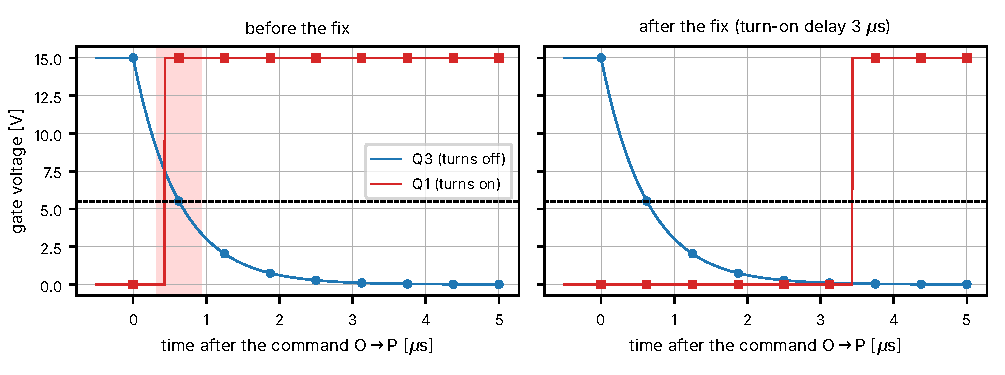
\includegraphics[width=\textwidth]{figures/fig_gate_timing.pdf}
\caption{Gate voltages at an O$\rightarrow$P change; markers: values at the steps of the local solver, dashed line: switch threshold. Left: before the fix (overlap at the first step, shaded). Right: with the turn-on delay of \SI{3}{\micro s}.}
\label{fig:gates}
\end{figure}

% =====================================================================================================
\section{Verification}
\label{sec:verification}

The companion script simulates the whole chain for \SI{1.5}{s} at vector level: shaft speed of \code{fixed\_speed\_setting} (step to the rated speed at \SI{25}{ms} through a \SI{0.1}{s} lag), torque curve with the \SI{1}{Hz} speed filter, current reference on the q axis, currents and DC voltages sampled, quantized ($2^{-11}\pu$) and one step late, control clock 1.001, the predictive control as a line-by-line copy of \code{mpc\_ttype\_gate} (checked against an Octave run of the MATLAB code), the EKF rebuilt block by block with the double integrator observer, and the encoder-sensorless switch. The plant is the machine in the rotor frame ($L_d$, $L_q$ plus the inductor), the T-type bridge with ideal switches and the \SI{3}{\micro s} turn-on delay (fixed model), the split DC link and the battery (open-circuit voltage, $R_0$, $R_1 \parallel C_1$). The gate filter and the Simscape solver are not modelled (the gate timing is checked apart on the solver grid, Sect.~\ref{sec:gates}). Table~\ref{tab:results} gives the averages over 1.2--\SI{1.5}{s}; Fig.~\ref{fig:startup}, \ref{fig:np} and \ref{fig:current} show the start-up, the neutral point and the current.

\begin{table}[!htb]
\centering
\caption{Results of the check (\SI{17.8}{rpm} unless stated; values over 1.2--\SI{1.5}{s}). Angle: error of the control angle; speed: estimate over true speed; torque: against the torque curve at the true speed; current error: rms over the two axes; switching: per device.}
\label{tab:results}
\small
\setlength{\tabcolsep}{4pt}
\begin{tabular}{llccccccc}
\toprule
 & Case & angle & speed & torque & current error & max $|v_{dc1} - v_{dc2}|$ & leg at O & switching \\
\midrule
A & before the fix & \ang{-21.6} & 0.982 & \SI{-11.5}{\percent} & 0.024 pu & \SI{80}{V} & \SI{8.5}{\percent} & \SI{1467}{Hz} \\
N1 & fixed, sensorless & \ang{-1.2} & 0.999 & \SI{-0.4}{\percent} & 0.008 pu & \SI{8}{V} & \SI{47}{\percent} & \SI{1532}{Hz} \\
N2 & fixed, encoder & \ang{-0.7} & 0.999 & \SI{0.0}{\percent} & 0.008 pu & \SI{9}{V} & \SI{46}{\percent} & \SI{1546}{Hz} \\
N3 & N1 without dead time & \ang{-1.2} & 0.999 & \SI{-0.4}{\percent} & 0.008 pu & \SI{9}{V} & \SI{46}{\percent} & \SI{1569}{Hz} \\
N4 & N1, machine $L$ \SI{+20}{\percent} & \ang{-10.6} & 0.999 & \SI{0.0}{\percent} & 0.008 pu & \SI{8}{V} & \SI{46}{\percent} & \SI{1559}{Hz} \\
N5 & N1, machine $L$ \SI{-15}{\percent} & \ang{+6.2} & 0.999 & \SI{-2.6}{\percent} & 0.009 pu & \SI{9}{V} & \SI{46}{\percent} & \SI{1549}{Hz} \\
N6 & N1, DC-link $C$ \SI{-50}{\percent} & \ang{-1.2} & 0.999 & \SI{-0.4}{\percent} & 0.008 pu & \SI{17}{V} & \SI{45}{\percent} & \SI{1598}{Hz} \\
N7 & N1 at \SI{12}{rpm} & \ang{-0.7} & 0.999 & \SI{-0.3}{\percent} & 0.004 pu & \SI{11}{V} & \SI{51}{\percent} & \SI{1429}{Hz} \\
N8 & N1, machine $L$ \SI{-20}{\percent} & lost & 0.999 & \SI{-6.4}{\percent} & 0.039 pu & \SI{32}{V} & \SI{37}{\percent} & \SI{1424}{Hz} \\
N9 & N8 with encoder & \ang{-0.7} & 0.999 & \SI{0.0}{\percent} & 0.009 pu & \SI{9}{V} & \SI{48}{\percent} & \SI{1651}{Hz} \\
S3 & N1, speed from the EKF state & \ang{-1.2} & 0.994 & \SI{-2.7}{\percent} & 0.008 pu & \SI{9}{V} & \SI{47}{\percent} & \SI{1524}{Hz} \\
D1 & N1 with $k_{dc} = 0$ & \ang{-1.1} & 0.999 & \SI{-0.4}{\percent} & 0.008 pu & \SI{147}{V} & \SI{52}{\percent} & \SI{968}{Hz} \\
\bottomrule
\end{tabular}
\end{table}

The fixed control puts the torque on the torque curve within \SI{0.4}{\percent} (sensorless) and cuts the current error to one third; the legs are at O about half of the time, as a carrier modulation would give for the same phase voltage ($1 - 2m/\pi = \SI{52}{\percent}$ with $m = \SI{476}{V}/(\SI{1275}{V}/2) = 0.75$). The remaining angle error is the age of the control angle (one step with the encoder, about two with the EKF, Sect.~\ref{sec:open}). The control does not depend on the dead time (N3) and keeps the neutral point with half the capacitance (N6). The sensorless control works with the machine inductances from \SI{-15}{\percent} to \SI{+20}{\percent} of the data; at \SI{-20}{\percent} the EKF loses the angle after about \SI{1}{s} (N8) while the control with the encoder still works (N9).

\begin{figure}[!htb]
\centering
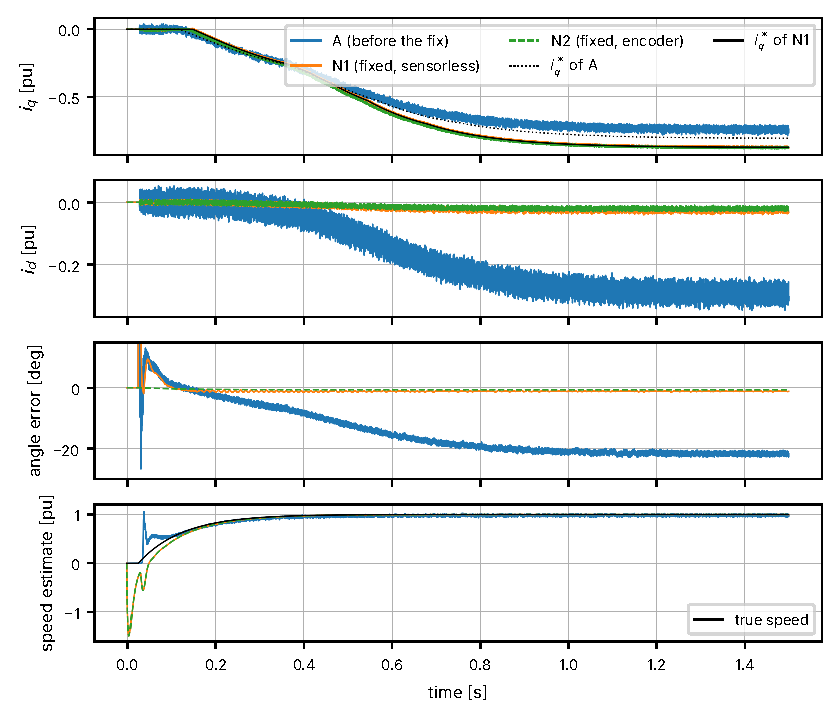
\includegraphics[width=0.8\textwidth]{figures/fig_startup.pdf}
\caption{Start-up and rated operation: q and d current, error of the control angle and speed estimate; model before the fix (A) and fixed model, sensorless (N1) and with the encoder (N2).}
\label{fig:startup}
\end{figure}

\begin{figure}[!htbp]
\centering
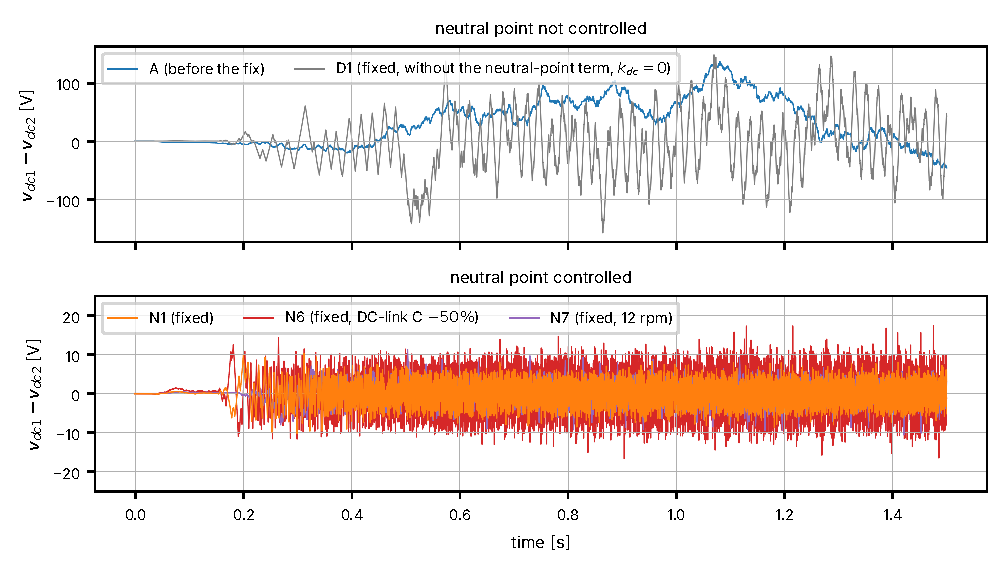
\includegraphics[width=\textwidth]{figures/fig_neutral_point.pdf}
\caption{Voltage difference of the two DC-link capacitors. Top: neutral point not controlled, before the fix (A) and fixed model without the neutral-point term (D1). Bottom: fixed model at rated speed (N1), with half the capacitance (N6) and at \SI{12}{rpm} (N7).}
\label{fig:np}
\end{figure}

\begin{figure}[!htbp]
\centering
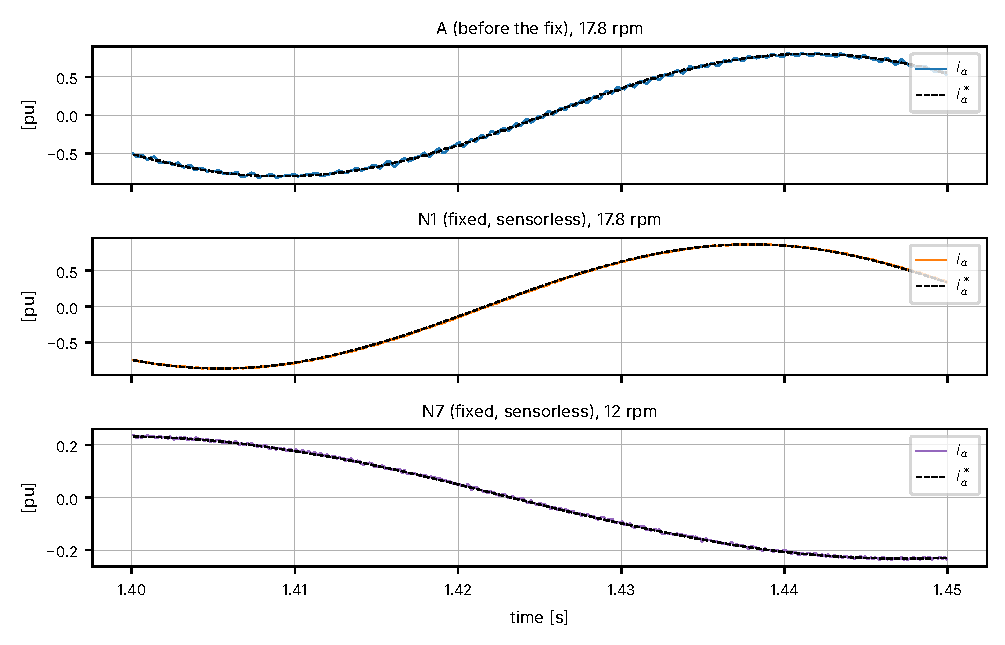
\includegraphics[width=\textwidth]{figures/fig_current_zoom.pdf}
\caption{Current $i_\alpha$ and its reference over \SI{50}{ms}: before the fix, fixed at rated speed and at \SI{12}{rpm}.}
\label{fig:current}
\end{figure}
\clearpage

% =====================================================================================================
\section{Remaining points}
\label{sec:open}

\begin{enumerate}
\item \textbf{Simulation in MATLAB.} The fixes were designed with the companion script and the parameters checked in Octave; the fixed model then ran well in MATLAB/Simulink. What the check predicts for the scopes: no short-circuit peak in the current of Q3 at an O$\rightarrow$P change, $v_{dc1} - v_{dc2}$ within about \SI{\pm 10}{V}, the torque on the torque curve, and the observers in agreement.
\item \textbf{Age of the control angle.} The angle is one step old with the encoder and about two steps old with the EKF, and the reference is the target of the next step: the current lags the rotor frame by \ang{1.4} to \ang{1.9}, $i_d \approx -0.02$ to $-0.03\pu$. An angle advance of $(n+1)\,\omega\ts$ in the current reference would remove it; the torque error is already below \SI{0.5}{\percent}.
\item \textbf{Sensorless range.} The EKF uses $L_q + L_{Fi}$ of the data; if the real inductances are not known within about \SI{\pm 15}{\percent} an adaptation of the inductance or of the angle is needed.
\item \textbf{Control clock.} The gain 1.001 of the control clock makes the prediction step \SI{0.1}{\percent} short and is the last error of the speed estimate; the alignment loop that should correct it has zero gains.
\item \textbf{DC voltage.} The battery holds the DC link at 1249--\SI{1275}{V}, 1.17--1.19 times $\udcn$ of the \SI{690}{V} data set: the voltage rating of the switches should be checked. The control uses the measured $v_{dc1}$, $v_{dc2}$.
\item \textbf{Bridge block.} The model still uses the old T-type bridge block of the library; the move to the new \code{semiconductors\_bridges} blocks is left to the planned migration of all models.
\end{enumerate}

% =====================================================================================================
\begin{thebibliography}{9}
\bibitem{kouro2009} S.~Kouro, P.~Cortés, R.~Vargas, U.~Ammann, J.~Rodríguez, ``Model predictive control---a simple and powerful method to control power converters,'' \emph{IEEE Trans. Ind. Electron.}, vol.~56, no.~6, pp.~1826--1838, 2009.
\bibitem{rodriguez2012} J.~Rodríguez, P.~Cortés, \emph{Predictive Control of Power Converters and Electrical Drives}, Wiley--IEEE Press, 2012.
\bibitem{cortes2012} P.~Cortés, J.~Rodríguez, C.~Silva, A.~Flores, ``Delay compensation in model predictive current control of a three-phase inverter,'' \emph{IEEE Trans. Ind. Electron.}, vol.~59, no.~2, pp.~1323--1325, 2012.
\bibitem{vargas2007} R.~Vargas, P.~Cortés, U.~Ammann, J.~Rodríguez, J.~Pontt, ``Predictive control of a three-phase neutral-point-clamped inverter,'' \emph{IEEE Trans. Ind. Electron.}, vol.~54, no.~5, pp.~2697--2705, 2007.
\bibitem{bolognani1999} S.~Bolognani, R.~Oboe, M.~Zigliotto, ``Sensorless full-digital PMSM drive with EKF estimation of speed and rotor position,'' \emph{IEEE Trans. Ind. Electron.}, vol.~46, no.~1, pp.~184--191, 1999.
\bibitem{boldea2008} I.~Boldea, M.~C.~Paicu, G.-D.~Andreescu, ``Active flux concept for motion-sensorless unified AC drives,'' \emph{IEEE Trans. Power Electron.}, vol.~23, no.~5, pp.~2612--2618, 2008.
\bibitem{schweizer2013} M.~Schweizer, J.~W.~Kolar, ``Design and implementation of a highly efficient three-level T-type converter for low-voltage applications,'' \emph{IEEE Trans. Power Electron.}, vol.~28, no.~2, pp.~899--907, 2013.
\end{thebibliography}

\end{onehalfspace}
\end{document}
